\documentclass{beamer}

%\frame{
%    \frametitle{}    
%    \begin{itemize}
%        \item<1->[] 
%        \item<2->[] 
%        \item<3->[] 
%    \end{itemize}
%}

% \usepackage{beamerthemesplit} // Activate for custom appearance
\usepackage{amsmath}
\usepackage{amssymb}
\usepackage{physics}
\usepackage{graphicx}
\usepackage{subcaption}



\title{The Fractal Inverse Problem For Audio Compression}
\author{Martin Pham}
\date{December 2017}

\begin{document}

\frame{\titlepage}

\frame{
    \begin{description}
		\item Introduction
		\item Motivating Example: Barnsley Fern
		\item Fractal Inverse Problem as Compression
		\item Further Directions
    \end{description}
}

\frame{
\begin{center}
"Fractal geometry will make you see everything differently. You risk the loss of your childhood vision of clouds, forests, galaxies, leaves, feathers, flowers, rocks, mountains, torrents of water, carpets, bricks, and much else besides. Never again will your interpretation of these things be quite the same." -Michael Barnsley
\end{center}
}

\frame{
	\begin{center}
		Consider a fractal as an object that exhibits \textbf{self-similarity} and \textbf{scale-free complexity}\\
	\end{center}
}

\frame{
	\frametitle{Sierpinski Carpet}
        \begin{figure}
          \centering
          \includegraphics[width=\linewidth]{sierpinskicarpet_1}
        \end{figure}
}
\frame{
	\frametitle{Sierpinski Carpet}
        \begin{figure}
          \centering
          \includegraphics[width=\linewidth]{sierpinskicarpet_2}
        \end{figure}
}
\frame{
	\frametitle{Sierpinski Carpet}
        \begin{figure}
          \centering
          \includegraphics[width=\linewidth]{sierpinskicarpet_3}
        \end{figure}
}

\frame{
        \begin{figure}
          \centering
          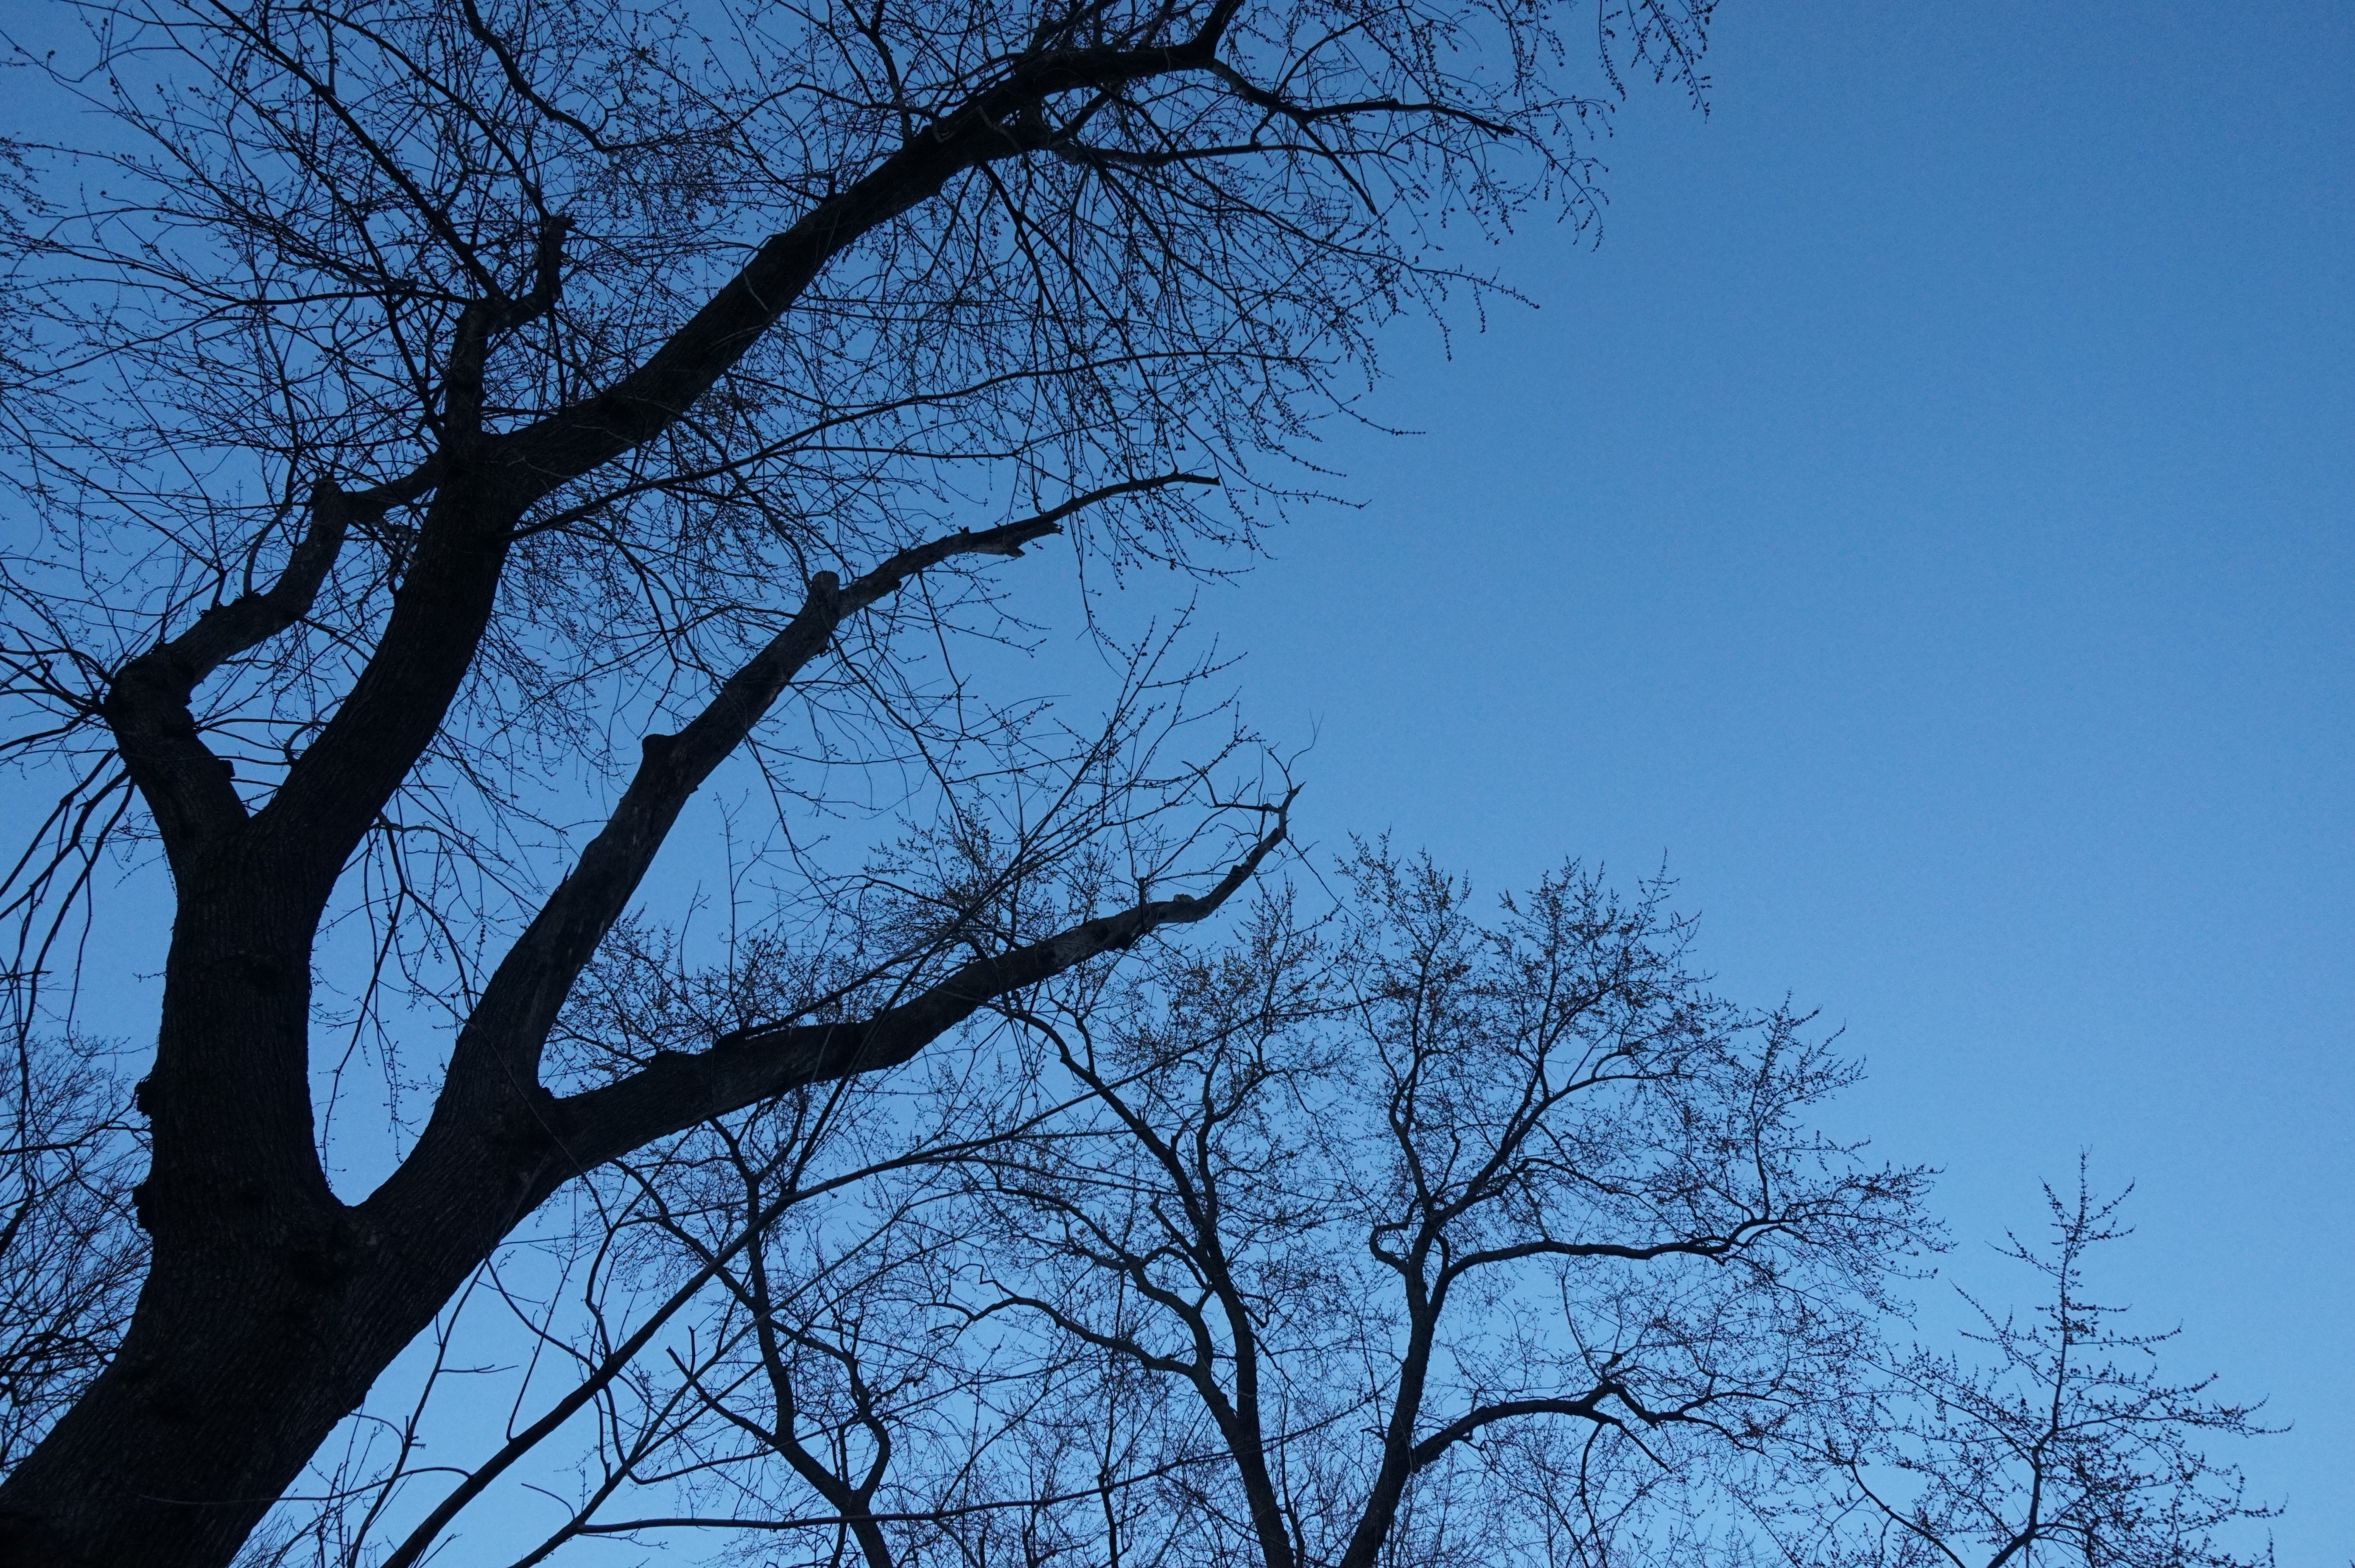
\includegraphics[width=\linewidth]{chicagotrees}
        \end{figure}
}

\frame{
	\frametitle{Introduction: IFS}
    \begin{itemize}
        \item<1->[] Michael Barnsley (1981) introduced iterated function systems (IFS) as a method for generating fractal objects
        \item<2->[] A set of contractive mappings on a complete metric space defines an IFS
        \item<3->[] The IFS defines an associated Hutchinson operator
    \end{itemize}
}

\frame{
	\frametitle{Introduction: Hutchinson operator}
    \begin{itemize}
        \item<1->[] The operator provides a notion of "combining" the actions of the set of mappings
        \item<2->[] It has an attractive fixed point, called a fractal because it is invariant under the operator (i.e. self-similarity)
    \end{itemize}
}

\frame{
	\begin{itemize}
	\item<1->[] Within nature, nothing has entirely scale-free complexity\\
	\item<2->[] Can't expect the form of a tree to infinitely scale down, at some point it becomes a biological cell\\
	\item<3->[] The same may be said for images and audio signals
    	\end{itemize}
}
\frame{
	\begin{itemize}
	\item<1->[] Local IFS method is more forgiving, suspends scale-free complexity at your desired resolution\\
	\item<2->[] Use larger subsections of a signal in order to approximate smaller subsections via a contractive affine transformation\\
	\end{itemize}
}

\frame{
	\frametitle{Introduction: Inverse Problem}

	\begin{itemize}
	\item<1->[] {Fractal compression may be posed as an inverse problem:\\
	\begin{center}
		\textbf{What set of parameters defines an IFS with a fixed point that well approximates our compression target?}
	\end{center}}
	\item<2->[] This is different from other lossy compression, where an appropriate representation reduces redundancy of information
	\item<3->[] Here, we seek a \textit{process} that will allow us to recover the target, not a \textit{representation} with fewer degrees of freedom
	\end{itemize}
}

\frame{
	\begin{center}
	Like looking for a treasure and having a map where no matter where you go you get to it
	\end{center}
}

% MOTIVATING EXAMPLE: GENERATING FRACTALS BY IFS
\frame{
    \begin{description}
		\item Introduction
		\item \textbf{Motivating Example: Barnsley Fern}
		\item Fractal Inverse Problem as Compression
		\item Further Directions
    \end{description}
}
\frame{
	\frametitle{Example: Barnsley Fern}
        Consider 4-map IFS with probabilities on $([-3,3]\times[0,10],\norm{\cdot})$
        \begin{small}
        \begin{align*}
	        w_{1}(x) &= \begin{bmatrix} 0&0 \\ 0&0.16 \end{bmatrix} x ,\qquad\qquad\qquad\quad p_1 = 0.01\\
		w_{2}(x) &= \begin{bmatrix} 0.85&0.04\\ -0.04&0.85 \end{bmatrix} x + \begin{bmatrix} 0 \\ 1.6 \end{bmatrix} ,\quad p_2 = 0.85\\
		w_{3}(x) &= \begin{bmatrix} 0.2&-0.26\\ 0.23&0.22 \end{bmatrix} x + \begin{bmatrix} 0 \\ 1.6 \end{bmatrix} ,\quad p_3 = 0.07\\
		w_{4}(x) &= \begin{bmatrix} -0.15&0.28\\ 0.26&0.24 \end{bmatrix} x + \begin{bmatrix} 0 \\ 0.44 \end{bmatrix} ,\quad p_4 = 0.07
        \end{align*}
        	\end{small}
}
\frame{
	The associated Hutchinson operator $T$ is then
	\[ (Tu)(x) =  \sum_{i=1}^{N} p_{i} u(w_{i}^{-1}(x)) \]
	This is a contractive operator that is guaranteed to have an attractive fixed point
	\[ \bar{u}(x) = (T\bar{u})(x) \]
	It is this fractal object $\bar{u}$ that we will want to well approximate our target, we will seek the mappings that define $T$
}

\frame{
	\begin{center}
	The Barnsley Fern Attractor\\
	(Demo)
	\end{center}
}

\frame{
	\begin{center}
	So given some IFS we can repeatedly apply our operator to obtain an associated fractal object, but how can we construct such an IFS to give us what we want?
	\end{center}
}
% LOCAL IFS AUDIO COMPRESSION ALGORITHM: INVERSE PROBLEM FOR ATTRACTORS
\frame{
    \begin{description}
		\item Introduction
		\item Motivating Example: Barnsley Fern
		\item \textbf{Fractal Inverse Problem as Compression}
		\item Further Directions
    \end{description}
}
\frame{
	Local IFS method (Jacquin, 1989) relaxes the global self-similarity constraint, requiring only a larger subsection of a signal to approximate a smaller subsection via a contractive transformation
        \begin{figure}
          \centering
          \includegraphics[width=\linewidth]{domainrange}
        \end{figure}
}

\frame{
	\begin{center}
	Lena\\(Demo)
	\end{center}
}

\frame{
\begin{figure}
        \begin{minipage}[b]{0.45\linewidth}
            \centering
            \includegraphics[width=\textwidth]{lena}
            \caption*{Uncompressed}
        \end{minipage}
        \hspace{0.5cm}
        \begin{minipage}[b]{0.45\linewidth}
            \centering
            \includegraphics[width=\textwidth]{lena_comp}
            \caption*{Compressed (15:1)}
        \end{minipage}
    \end{figure}
}

\frame{
	\begin{itemize}
	\centering
	\item<1->[] Can the same be performed for one-dimensional signals?
	\item<2->[] Yes
	\end{itemize}
}

\frame{
	\frametitle{An Audio Fractal Encoder in Space}
	Encoding:
	\begin{itemize}
	\item Divide signal into two sets of range blocks with length $N$ bits and domain blocks of length $2N$ bits
	\item For each range block, find the domain block and transformation that best approximates the current range block
	\item Save the domain block index and contractive mapping that best approximates that range block
	\item This defines the operator that is saved as an encoded file
	\end{itemize}
}
\frame{
	\frametitle{An Audio Fractal Encoder in Space}
	Decoding:
	\begin{itemize}
	\item Start with \textit{any} signal of appropriate length
	\item Divide signal into two sets of range blocks with length $N$ bits and domain blocks of length $2N$ bits
	\item For each range block, get the associated encoded domain block index and contractive mapping
	\item Replace the range blocks with the approximations by the domain blocks
	\item Repeat application of operator until residual is below some desired threshold
	\end{itemize}
}
\frame{
	\begin{center}
	Compression ratio of 2.7:1\\or\\What does a fractal sound like?
	\end{center}
}

% FURTHER DIRECTIONS
%\frame{
%    \begin{description}
%		\item Introduction
%		\item Motivating Example: Barnsley Fern
%		\item Fractal Inverse Problem as Compression
%		\item \textbf{Further Directions}
%    \end{description}
%}
%\frame{
%	\frametitle{Limitations}
%	\begin{itemize}
%	\item<1->[] Frequency artefacts added by discontinuities between blocks
%	\item<2->[] Global search for affine transformations associated to the best domain block is of quadratic order
%	\end{itemize}
%}
%\frame{
%	\frametitle{Some Potential Solutions}
%	Frequency artefacts may be reduced by
%	\begin{itemize}
%	\item Overlapping tessellation of range blocks
%	\item Higher order or non-linear contractive mappings
%	\item Post-processing in order to smooth out signal across blocks
%	\end{itemize}
%}
%\frame{
%	Unclear if there are any robust and efficient search methods\\
%	Some things to consider however:
%	\begin{itemize}
%	\item Audio signals may be smoother but much less flat than images
%	\item Incorporate some psychoacoustical techniques
%	\item Other spaces of representation induce a fractal transform in those spaces
%	\end{itemize}
%}


\frame{
	\frametitle{Further Directions: Wavelets}
	\begin{itemize}
	\item<1->[] A wavelet multiresolution analysis (Mallat, 1989) of the signal provides a representation that is amenable to fractal methods
	\item<2->[] Wavelets have both a frequency and spatial component, and may be represented in the form of coefficient trees
	\item<3->[] These trees are self-similar and so compression may be formed as a fractal inverse problem on wavelet coefficients
	\end{itemize}
}
\frame{
	\begin{itemize}
	\item<1->[] Previous work (Wannamaker, 1997) has yielded a fractal-wavelet approach with up to $6:1$ compression ratio
	\item<2->[] Working in the wavelet domain opens up many more options for search and encoding strategies
	\end{itemize}
}
\frame{
	\begin{center}
	Wavelet bases are usually constructed depending on application, perhaps a basis may be chosen depending on preliminary analysis of signal before encoding process
	\end{center}
}
\frame{
	The question becomes: 
	\begin{center}
	In what wavelet basis up to what level of resolution do we need for fractal-wavelet methods to achieve certain compression ratios with acceptable audio fidelity?
	\end{center}
}
\frame{
	Furthermore,
	\begin{center}
	What kind of domain blocks are used to approximate the most number of range blocks?
	\end{center}
}
\frame{
	\begin{center}
	Thanks
	\end{center}
}





\end{document}
